\subsection{Mockups}
Tras la aprobación de la propuesta por todas las partes implicadas se empieza a trabajar en el diseño de la aplicación. Teniendo en cuenta que la web será accesible tanto por dispositivos móviles como por ordenadores se realizan dos diseños distintos: una versión móvil y otra de escritorio. Ambas versiones siguen los mismos principios pero tratan de adaptarse al tamaño de pantalla y hacer un uso adecuado del espacio.\\

Como fuente veraz de información el servicio debe transmitir fiabilidad y confianza, por esta razón se opta por un estilo sobrio y sencillo donde diferentes tonos de azul predominan. Con ello se espera que transmita una sensación de paz y seguridad al usuario.\\

La aplicación se compone de tres pantallas distintas: selección del asistente, chat y consulta de información.\\

\subsubsection{Selección del asistente}
En busca de establecer un primer vínculo entre el chatbot y el usuario se dota al sistema de dos personalidades distintas para humanizar la experiencia. En la primera pantalla a través de dos avatares (Juan y Elena) (ver figura \ref{fig:mobile avatar} y \ref{fig:desktop avatar}) el usuario puede eligir con cual de estas dos identidades desea mantener una conversación y así empezar a crear la relación. Además de elegir con quién se siente más cómodo hablando, puede leer el aviso sobre el tratamiento de sus datos y pulsar "\textit{Empezar}" para aceptar los términos y proceder al chat.\\

\begin{figure}[htbp]
\centering
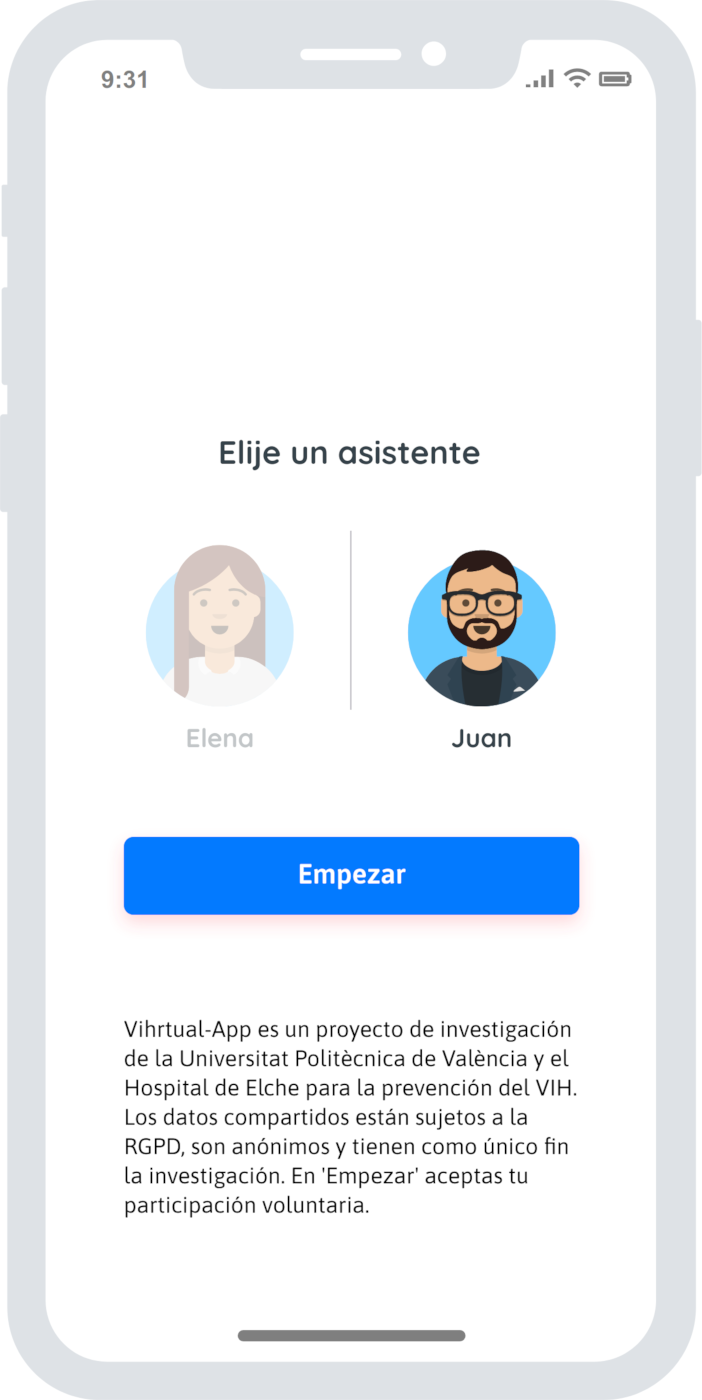
\includegraphics[scale=0.2]{../images/mobile_avatar.png} 
\caption{Selección del asistente. Versión móvil}
\label{fig:mobile avatar}
\end{figure}

\begin{figure}[htbp]
\centering
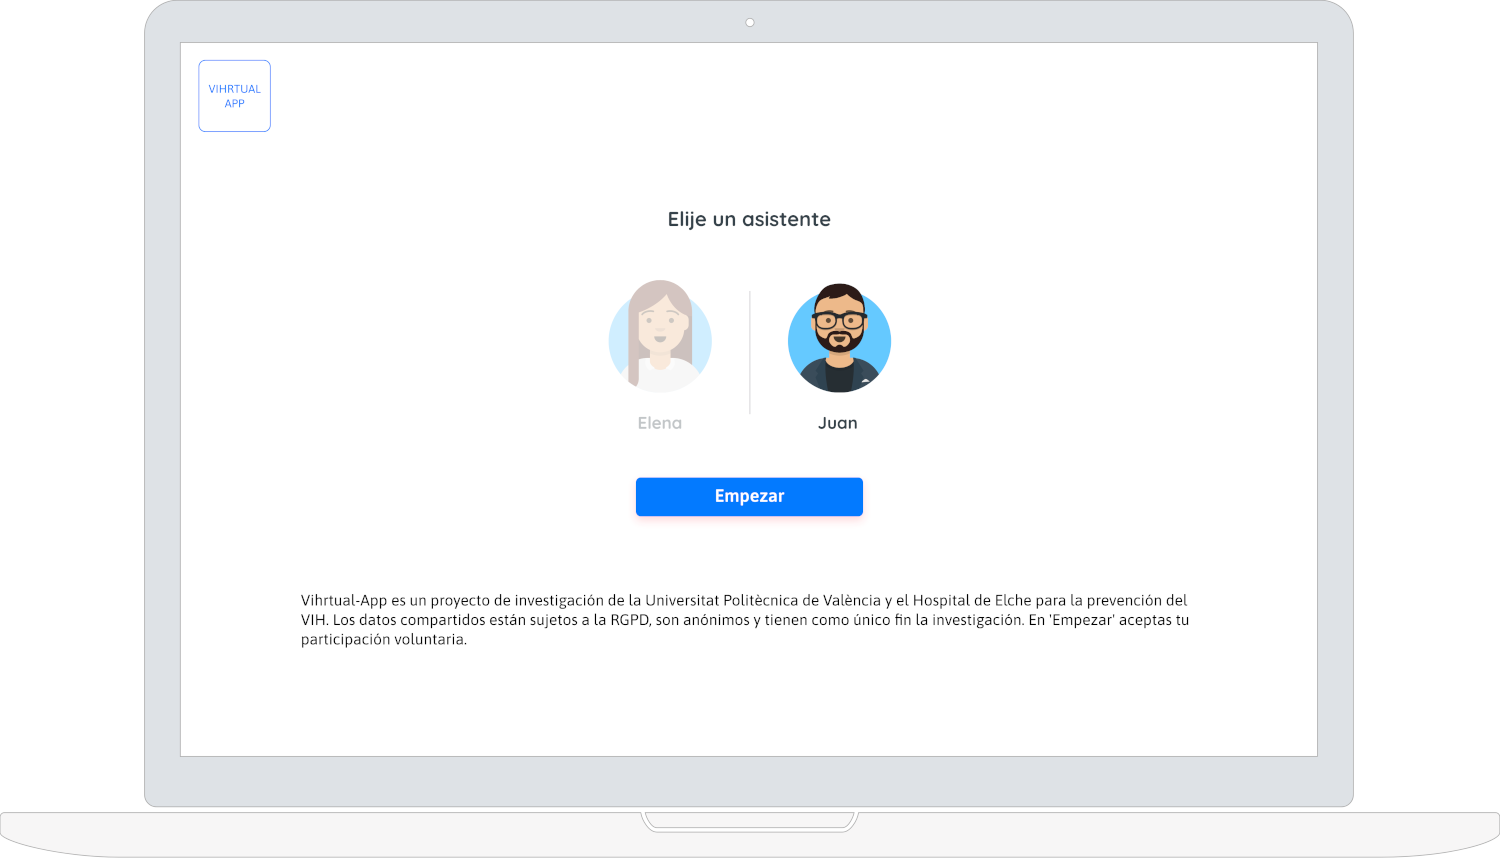
\includegraphics[scale=0.2]{../images/desktop_avatar.png} 
\caption{Selección del asistente. Versión de escritorio}
\label{fig:desktop avatar}
\end{figure}

\subsubsection{Chat}
Desde un principio se tiene claro que el diseño debe girar alrededor de la interacción con el \textit{bot}, y por tanto, el chat debe ser el elemento principal de la aplicación. Por ello, en la versión móvil se opta por una disposición donde prácticamente todo el espacio es ocupado por la conversación (ver figura \ref{fig:mobile chat}). En cambio, en la versión de escritorio el chat ocupa la mitad derecha de la pantalla, mostrando en la parte izquierda la imagen del avatar escogido con un pequeño texto informativo (ver figura \ref{fig:desktop chat}). El estilo del chat sigue los patrones de diseño típicos y más o menos estandarizados de aplicaciones de mensajería instantánea como \textit{WhatsApp} o \textit{Telegram}. El motivo detrás de esta decisión es facilitar la usabilidad ya que prácticamente la totalidad de los usuarios están familiarizados con este tipo de interfaces.\\

En la cabecera superior encontramos los elementos habituales: la imagen de perfil de con quién se está hablando y un pequeño texto que nos indica el estado: "\textit{en línea}" o "\textit{escribiendo ...}". Ambos elementos juegan una papel importante en la simulación: mientras la conversación transcurre el usuario ve constantemente el avatar del asistente e inconscientemente realiza una asociación entre los mensajes y la imagen de la persona que esta viendo. Por otra parte, aunque el usuario sepa que es una simulación observar como el chatbot va cambiando su estado según esté escribiendo o no vuelve a reforzar la idea debido al paralelismo con las aplicaciones anteriormente mencionadas.\\

Por último, a través del icono de la esquina superior derecha se accede a consultar la información.\\

\begin{figure}[htbp]
\centering
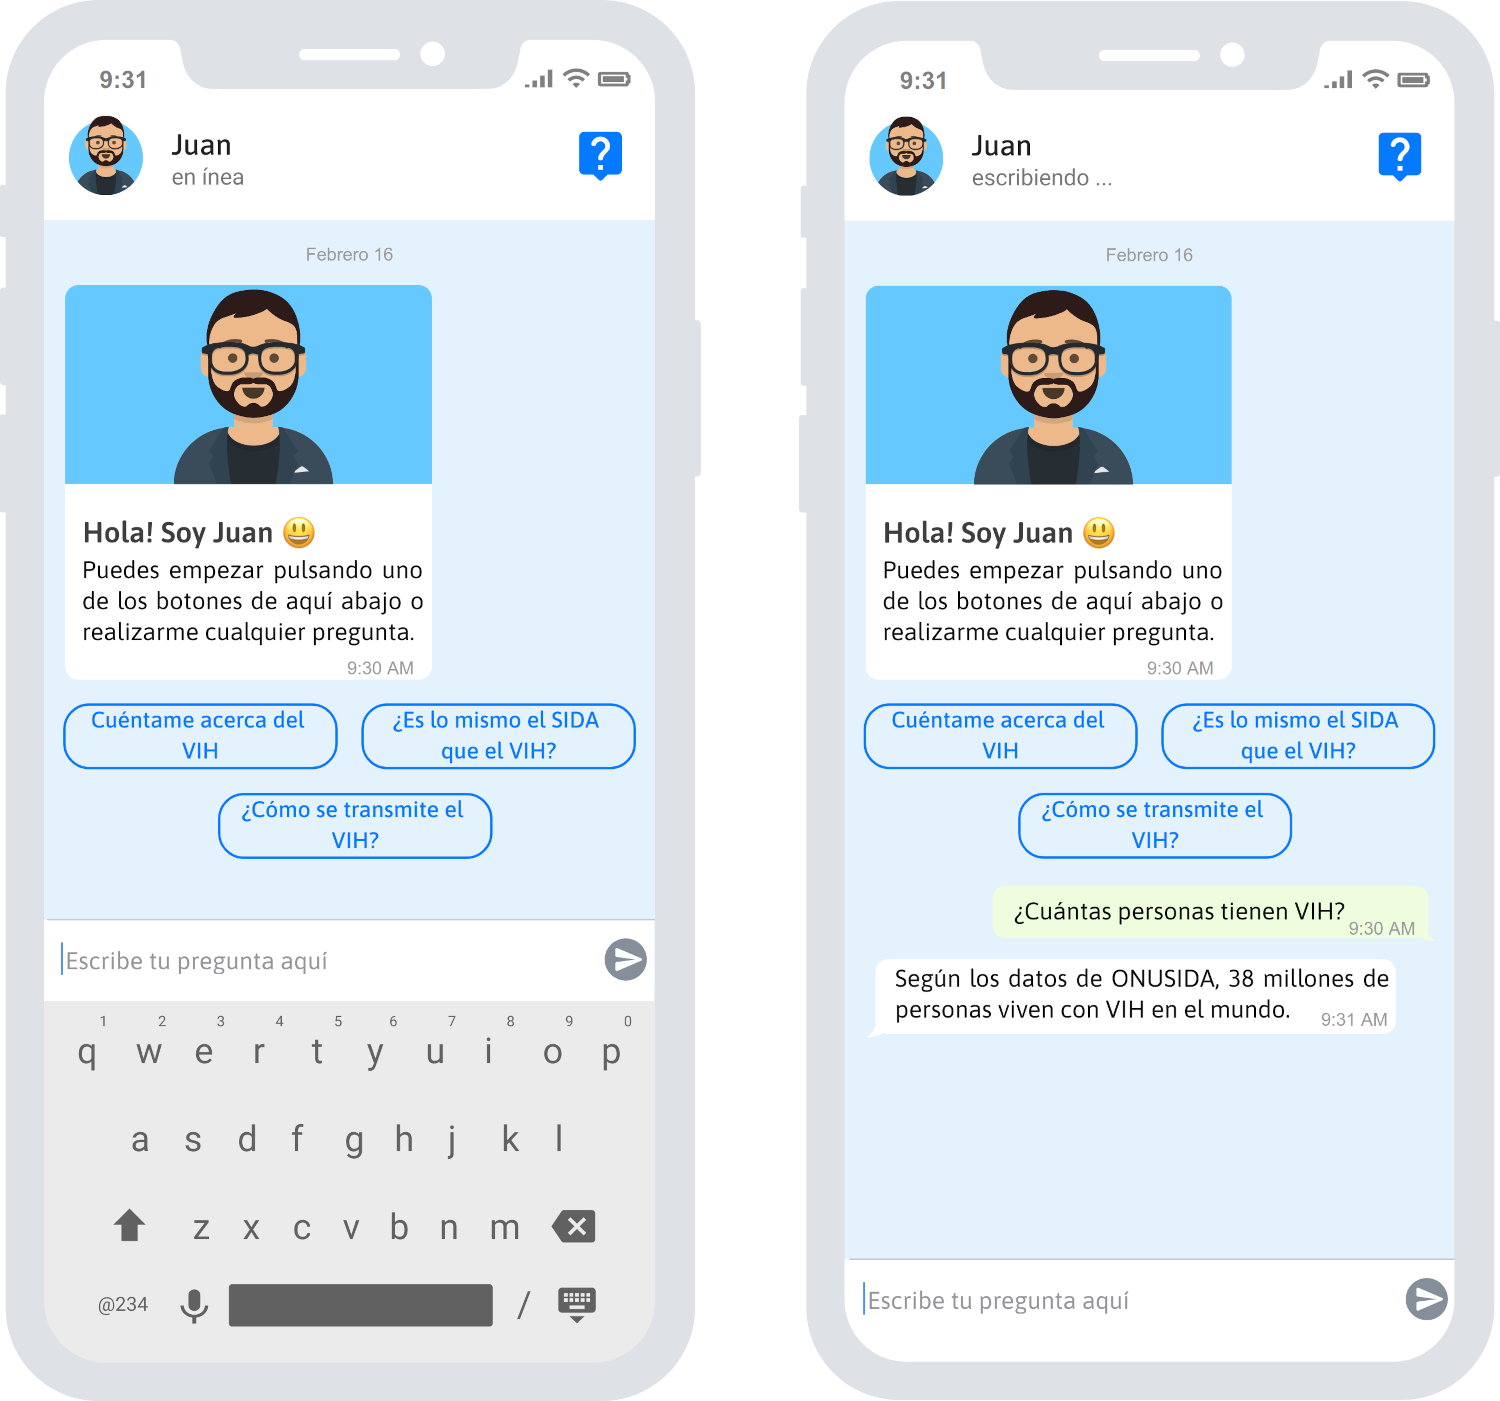
\includegraphics[scale=0.2]{../images/mobile_chat.png} 
\caption{Chat. Versión móvil}
\label{fig:mobile chat}
\end{figure}

\begin{figure}[htbp]
\centering
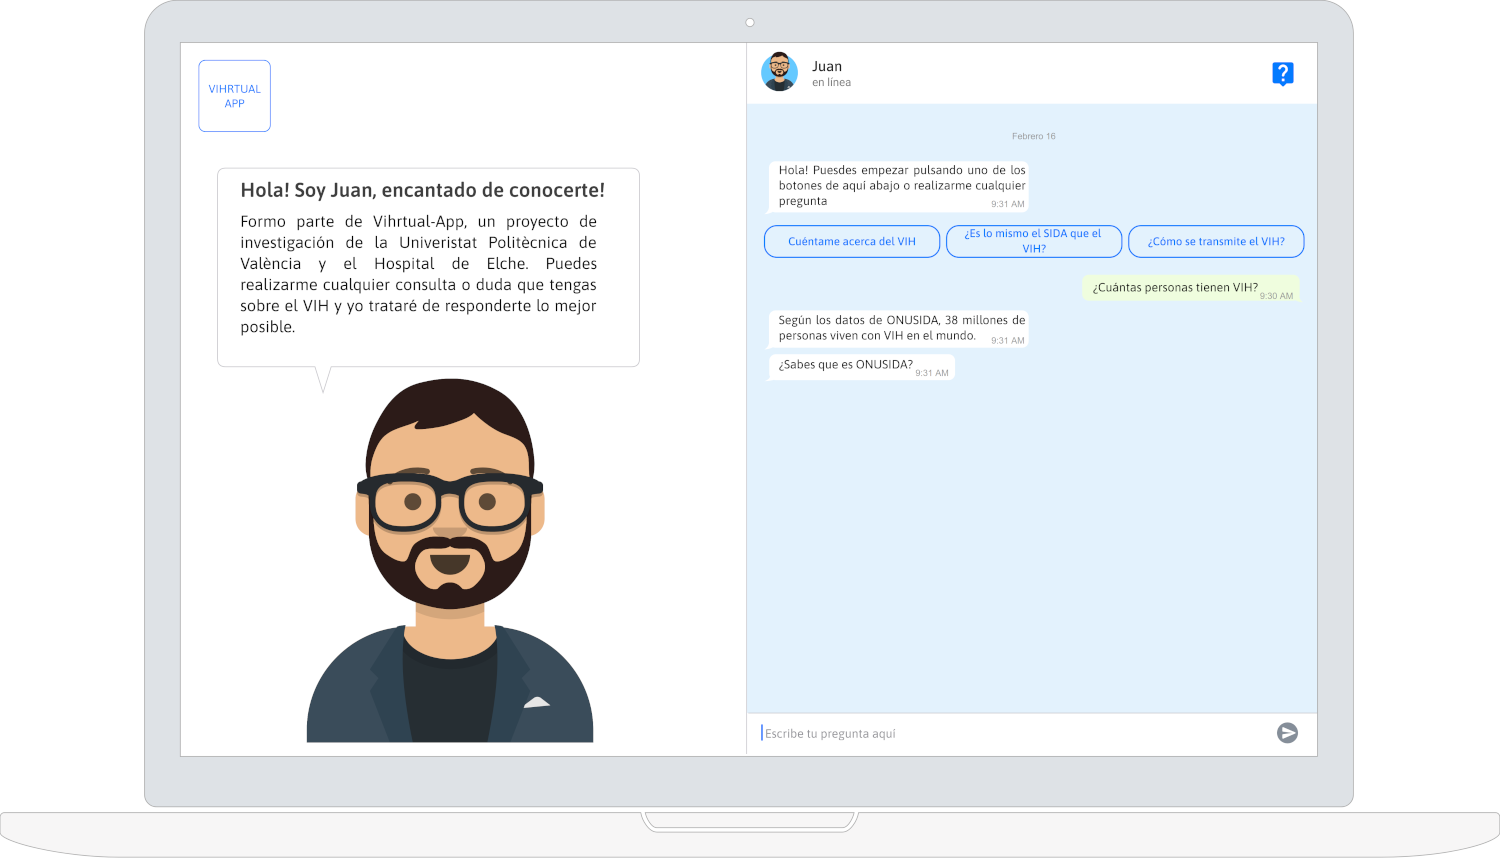
\includegraphics[scale=0.2]{../images/desktop_chat.png} 
\caption{Chat. Versión de escritorio}
\label{fig:desktop chat}
\end{figure}


\subsubsection{Consulta de información}
La pantalla de información contiene una breve introducción al VIH y una serie de temas anidados que se pueden ir desplegando y consultando. Además, en la parte superior existe una barra de búsqueda que permite encontrar rápidamente ciertos términos o palabras clave. Si existen resultados que coincidan con la búsqueda se indica con un pequeño indicador amarillo sobre el desplegable y resaltando el término en cuestión (ver figura \ref{fig:mobile search}).\\

\begin{figure}[htbp]
\centering
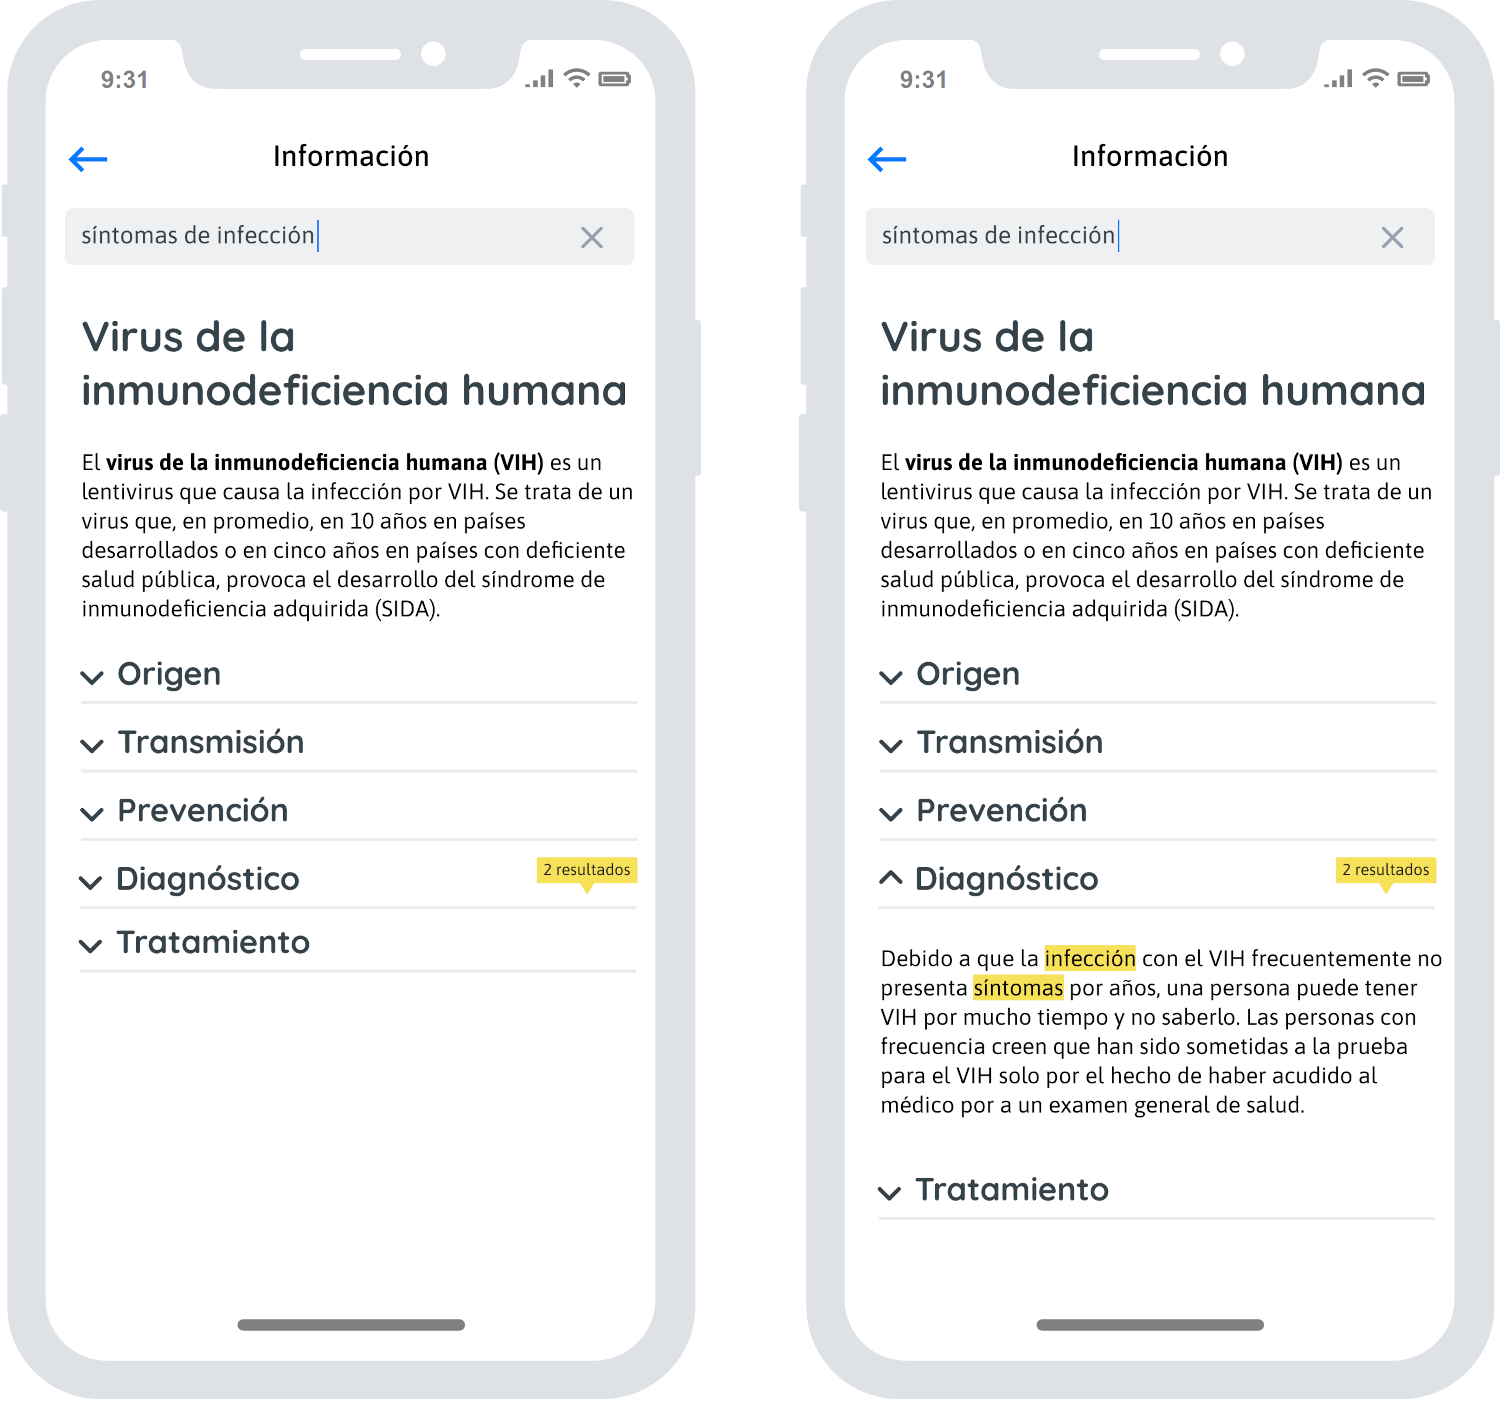
\includegraphics[scale=0.2]{../images/mobile_search.png} 
\caption{Búsqueda de información. Versión móvil}
\label{fig:mobile search}
\end{figure}

\begin{figure}[htbp]
\centering
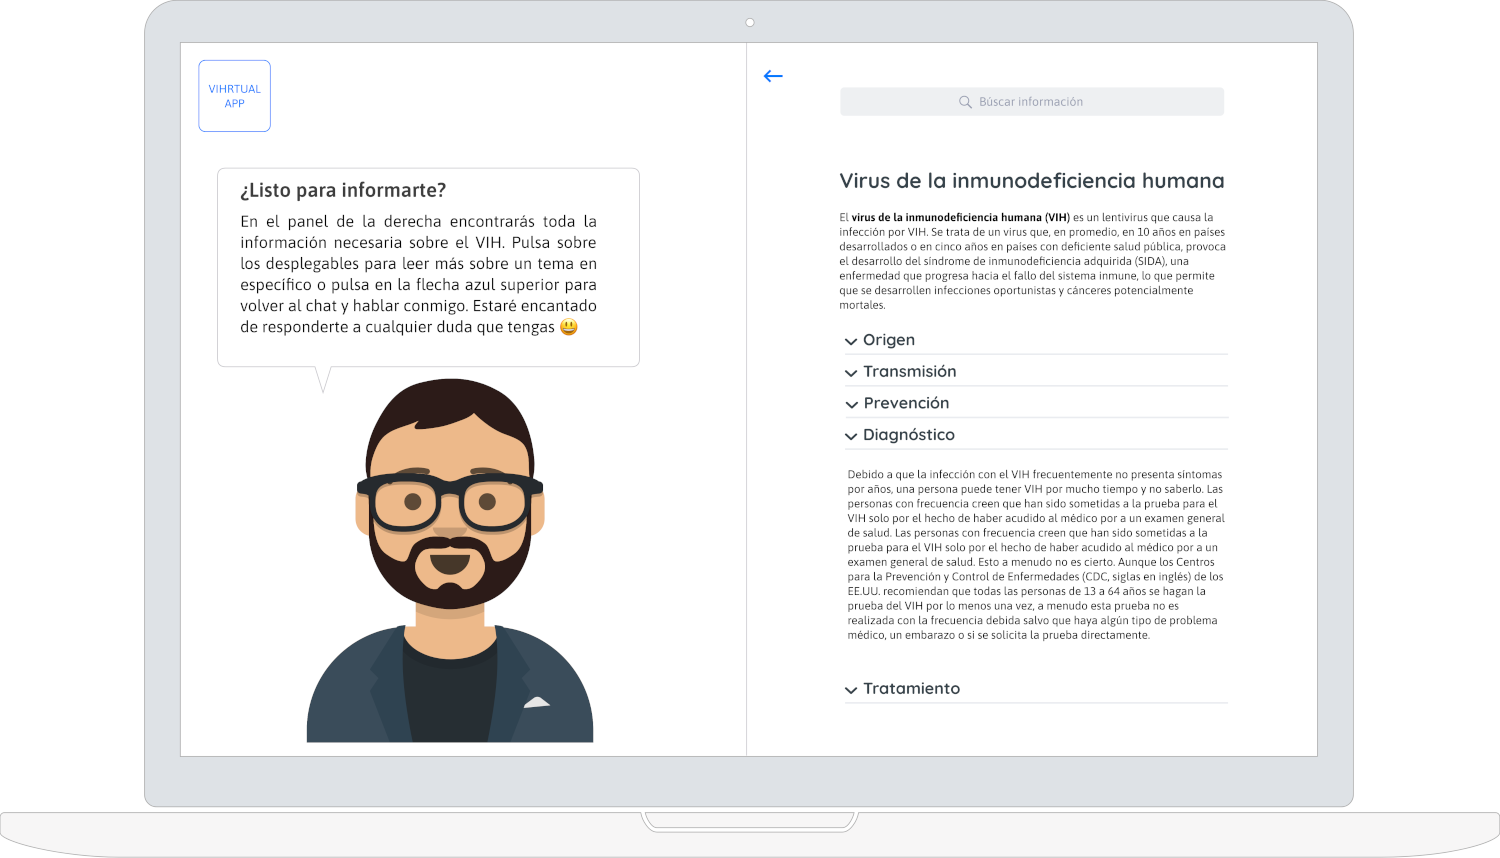
\includegraphics[scale=0.2]{../images/desktop_search.png} 
\caption{Búsqueda de información. Versión de escritorio}
\label{fig:mobile search}
\end{figure}

Estos \textit{mockups} se envían con un pequeño vídeo y encuesta a los colaboradores la Unidad de Enfermedades Infecciosas del Hospital General de Elche para obtener su \textit{feedback} y aprobación. Tanto sus indicaciones como la versión interactiva pueden encontrarse en los documentos anexos a este trabajo.\\



\begin{figure}[htbp]
\centering
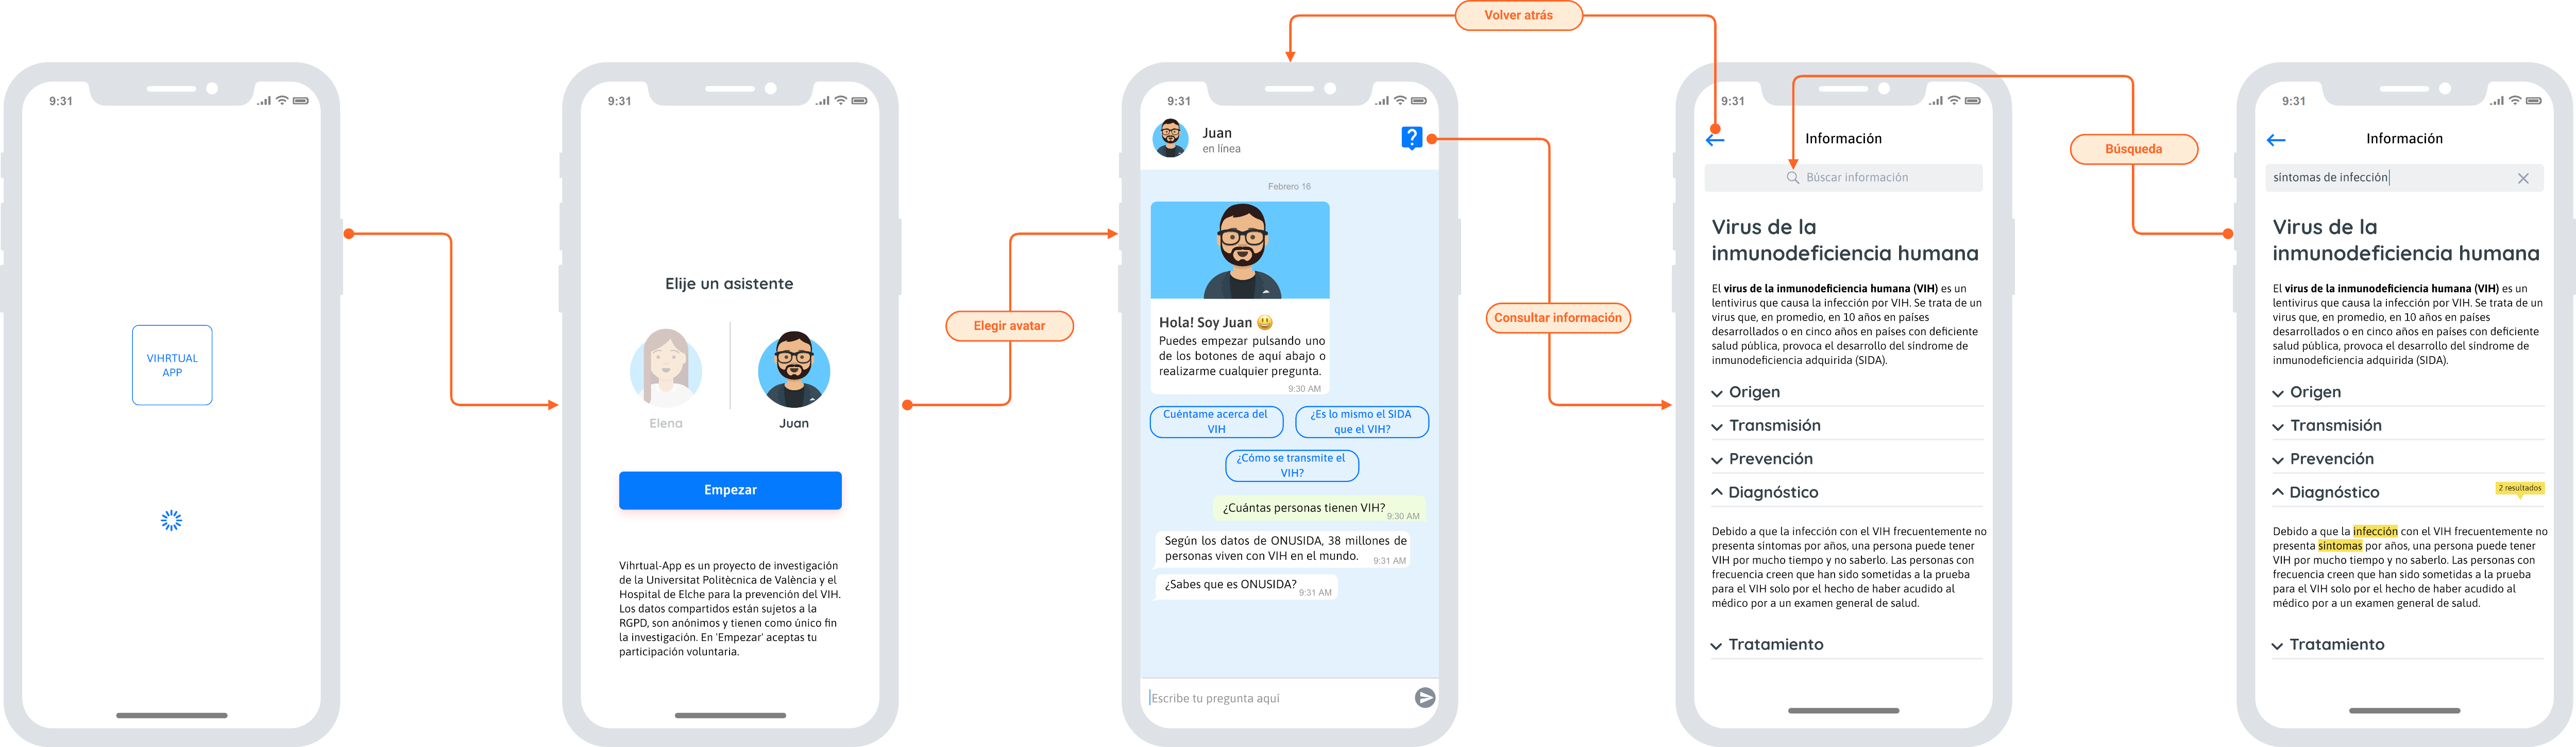
\includegraphics[scale=0.1]{../images/mobile_flow.png} 
\caption{Diagrama de navegación de la aplicación. Versión móvil}
\label{fig:mobile flow}
\end{figure}

\subsection{Diseño de diálogo}
[TODO: Dialog flow charts etc]


\subsection{Diseño de software y arquitectura}
[TODO: Diagramas del diseño de software y aquitectura de la aplicación]
